% !TEX encoding = UTF-8 Unicode
% !TEX TS-program = LuaLaTeX
% !TEX root = ../memoire.tex
% !TEX spellcheck = fr-FR

%************************************************
\chapter{Ensembles de classifieurs}
\label{chap:trois}
%************************************************

\todo{Comme algorithme de Base il faudrait choisir un arbre seul plutot qu'une foret}

\section{Décomposition biais-variance}\label{sec:biais.var}
\subsection{Dans le cas de la régression $L^2$}

On rappelle que l'erreur de prédiction à un certain point $X=x$ est:
\begin{equation}
    \operatorname{Err} (\varphi_{\mathcal{L}} (x) ) = \mathbb{E}_{Y \mid X = x} \left[ L(Y,\varphi_{\mathcal{L}} (x) ) \right]
\end{equation}
Dans le cas de la régression le choix le plus courant et naturel pour $L$ est la perte quadratique. On peut alors en notant $\varphi_B$ le modèle idéal théorique de Bayes:
\begin{align*}
    \operatorname{Err} (\varphi_{\mathcal{L}} (x) ) &= \mathbb{E}_{Y \mid X = x} \left[ (Y - \varphi_{\mathcal{L}} (x) )^2 \right]  \notag \\
    &= \mathbb{E}_{Y \mid X = x} \left[ (Y - \varphi_{B} (x) + \varphi_{B} (x) - \varphi_{\mathcal{L}} (x) )^2 \right]  \notag \\
    &= \mathbb{E}_{Y \mid X = x} \left[ (Y - \varphi_{B} (x) )^2 \right]  + \mathbb{E}_{Y \mid X = x} \left[ (\varphi_{B} (x) - \varphi_{\mathcal{L}} (x) )^2 \right]  \notag \\
    &+ \mathbb{E}_{Y \mid X = x} \left[ 2 (Y-\varphi_B (x) ) ( \varphi_B (x) - \varphi_{\mathcal{L}} (x) ) \right] \notag \\
    &= \operatorname{Err} \left(\varphi_{B} (x) \right) + \left( \varphi_{B} (x) - \varphi_{\mathcal{L}} (x) \right)^2
\end{align*}
Par définition du classifieur de Bayes on a $\mathbb{E}_{Y \mid X = x} \left[ Y - \varphi_B (x) \right] = 0$
Si de plus on considère que l'échantillon d'apprentissage $\mathcal{L}$ est une variable aléatoire et que l'algorithme d'apprentissage est déterministe, on peut écrire l'erreur moyenne due à l'échantillonnage
\begin{align}
    &\mathbb{E}_{\mathcal{L}} \left[ ( \varphi_B (x) - \varphi_{\mathcal{L}} (x) )^2 \right] \notag \\
    &= ( \varphi_B (x) - \mathbb{E}_{\mathcal{L}} [ \varphi_{\mathcal{L}} (x) ] )^2 + \mathbb{E}_{\mathcal{L}} \left[ ( \mathbb{E}_{\mathcal{L}} [ \varphi_{\mathcal{L}} (x) ] -  \varphi_{\mathcal{L}} (x) )^2 \right]
\end{align}
On obtient alors la décomposition biais-variance due à \citet{Geman1992}:
\begin{theoreme}[Décomposition biais-variance]
    Dans le cas de la perte $L^2$ on a:
    \begin{equation}
        \mathbb{E}_{\mathcal{L}} \left[ \operatorname{Err} ( \varphi_{\mathcal{L}} (x) ) \right] = \operatorname{bruit} (x) + \operatorname{biais}^2 (x) + \operatorname{var} (x)
    \end{equation}
    où
    \begin{align*}
        \operatorname{bruit} (x) &= \operatorname{Err} (\varphi_{B} (x) ) \\
        \operatorname{biais}^2 (x) &= ( \varphi_B (x) - \mathbb{E}_{\mathcal{L}} \left[ \varphi_{\mathcal{L}} (x) \right] )^2 \\
        \operatorname{var} (x) &= \mathbb{E}_{\mathcal{L}} \left[ \left( \varphi_{\mathcal{L}} (x) - \mathbb{E}_{\mathcal{L}} [ \varphi_{\mathcal{L}} (x) ] \right)^2 \right]
    \end{align*}
\end{theoreme}

\subsection{Extension à la classification binaire}

Dans le cas de la perte 0-1, c'est-à-dire 
\begin{equation*}
    \mathbb{E}_{\mathcal{L}} \left[ \mathbb{E}_{Y \mid X = x} [ \mathds{1}_{\varphi_{\mathcal{L}} (x) \neq Y } ] \right] = \mathbb{P}_{\mathcal{L},Y \mid X = x} ( \varphi_{\mathcal{L}} (x) \neq Y )
\end{equation*}
il est possible d'utiliser le fait que de nombreux algorithmes de classification calculent en réalité l'estimateur $ \hat{p}_{\mathcal{L}} ( Y = c \mid X = x ) $ et en déduisent la classe par la règle:
\begin{equation*}
    \varphi_{\mathcal{L}} (x) = \argmax_{c \in \mathcal{Y}} \hat{p}_\mathcal{L} ( Y = c \mid X = x )
\end{equation*}
On trouve alors de la même façon que précédemment la décomposition
\begin{align*}
    &\mathbb{E}_{\mathcal{L}} \left[ \mathbb{E}_{Y \mid X = x} \left[ \mathds{1}_{\varphi_{\mathcal{L}} (x) \neq Y } \right]  \right] \\
    &= \mathbb{P} \left( \varphi_B (x) \neq Y \right) + \mathbb{P}_{\mathcal{L}} \left( \varphi_{\mathcal{L}} (x) \neq \varphi_B (x) \right) \left( 2 \mathbb{P} \left( \varphi_B (x) = Y \right) - 1 \right)
\end{align*}
où $\mathbb{P}$ est à chaque fois $\mathbb{P}_{Y \mid X = x}$. La prévision du modèle diffère de la prévision optimale de Bayes lorsque
\begin{equation*}
    \mathbb{P}_{\mathcal{L}} \left( \varphi_{\mathcal{L}} (x) \neq \varphi_B (x) \right) = \mathbb{P}_{\mathcal{L}} \left( \hat{p}_{\mathcal{L}} (Y = \varphi_B (x) ) < 0.5 \right)
\end{equation*}

Si l'on suppose alors que $\hat{p}_{\mathcal{L}} (Y = \varphi_B (x))$ est normalement distribuée alors on obtient le théorème suivant
\begin{theoreme}[\cite{Louppe2014}]
Pour la perte 0-1 dans le cas de la classification, l'erreur de généralisation attendue $\mathbb{E}_{\mathcal{L}} \left[ \operatorname{Err} ( \varphi_{\mathcal{L}} (x) ) \right]$ en $ X = x $ admet la décomposition suivante:
\begin{gather*}
    \mathbb{E}_{\mathcal{L}} \left[ \operatorname{Err} ( \varphi_{\mathcal{L}} (x) ) \right] = \mathbb{P} ( \varphi_B (x) \neq Y ) + \dotsb \\
    \dotsb + \Phi \left( \frac{0.5 - \mathbb{E}_{\mathcal{L}} [ \hat{p}_{\mathcal{L}} (Y = \varphi_B (x)) ] }{\sqrt{\mathbb{V}_{\mathcal{L}} \hat{p}_{\mathcal{L}} (Y = \varphi_B (x)) } } \right) \left( 2 \mathbb{P} ( \varphi_B (x) = Y ) - 1 \right)
\end{gather*}
\end{theoreme}

On déduit de ce théorème deux cas importants:
\begin{itemize}
    \item Lorsque $\mathbb{E}_{\mathcal{L}} \left[ \hat{p}_{\mathcal{L}} (Y = \varphi_B (x)) \right] > 0.5$ alors une réduction de la variance réduit l'erreur vers l'erreur de Bayes.
    \item Lorsque $\mathbb{E}_{\mathcal{L}} \left[ \hat{p}_{\mathcal{L}} (Y = \varphi_B (x)) \right] < 0.5$ une réduction de la variance augmente l'erreur.
\end{itemize}

\section{Réduction de la variance}
\subsection{Combinaison linéaire de classifieurs}\label{subsec:combinaison_lineaire}

On suppose être capable de créer des classifieurs aléatoires $\varphi_{\mathcal{L},m}$ tous appris sur le même échantillon et prédisant le même modèle. On veut alors combiner ces classifieurs en \emph{ensemble de classifieurs} afin d'éventuellement réduire l'erreur de généralisation par rapport à un classifieur unique.
La méthode la plus naturelle pour agréger les prédictions des classifieurs est une combinaison linéaire des prédictions, ainsi dans le cas de la régression on adopte:
\begin{equation*}
    \psi_{\mathcal{L},1,\dotsc,M} (x) = \frac{1}{M} \sum_{m=1}^M \varphi_{\mathcal{L},m} (x)
\end{equation*}

Dans le cas de la classification, si les classifieurs ne fournissent que des prévisions 0-1 on utilise le \emph{vote de majorité} pour effectuer la prédiction finale
\begin{equation*}
     \psi_{\mathcal{L},1,\dotsc,M} (x) = \argmax_{c \in \mathcal{Y}} \frac{1}{M} \sum_{m=1}^M \mathds{1}_{\varphi_{\mathcal{L},m} (x) = c}
\end{equation*}
Dans le cas où les classifieurs donnent en sortie $\hat{p}_{\mathcal{L},m} ( Y = c \mid X = x)$ on peut adopter comme règle de vote
\begin{equation*}
     \psi_{\mathcal{L},1,\dotsc,M} (x) = \argmax_{c \in \mathcal{Y}} \frac{1}{M} \sum_{m=1}^M \hat{p}_{\mathcal{L},m} ( Y = c \mid X = x)
\end{equation*}

\todo{A faire dans le cas de la classification}

Il est alors possible de montrer le théorème suivant:
\begin{theoreme}[\cite{Louppe2014}]
        Dans le cas de la régression $L^2$, la décomposition biais-variance de l'erreur de généralisation attendue $\mathbb{E}_{\mathcal{L}} \left[ \operatorname{Err} \left( \psi_{\mathcal{L},1,\dotsc,M} (x) \right) \right] $ d'un ensemble de $M$ classifieurs aléatoires $\varphi_{\mathcal{L},m}$ est:
        \begin{equation*}
            \mathbb{E}_{\mathcal{L}} \left[ \operatorname{Err}(\psi_{\mathcal{L},1,\dotsc,M} (x)) \right] = \mathrm{bruit}(x) + \mathrm{biais}^2 (x) + \mathrm{var} (x)
        \end{equation*}
        avec
        \begin{align*}
            \mathrm{bruit}(x) &= \operatorname{Err} ( \varphi_B (x) ) \\
            \mathrm{biais}^2 (x) &= \left( \varphi_B (x) - \mathbb{E}_{\mathcal{L},i} \left[ \varphi_{\mathcal{L},i} (x) \right] \right)^2 \\
            \mathrm{var} (x) &= \rho (x) \sigma^2_{\mathcal{L},i} (x) + \frac{1-\rho (x)}{M} \sigma^2_{\mathcal{L},i} (x) 
        \end{align*}
        Avec
        \begin{gather*}
            \sigma^2_{\mathcal{L},i} (x) = \mathbb{V}_{\mathcal{L},i} [ \varphi_{\mathcal{L},i} (x)] \\
            \mu_{\mathcal{L},i} (x) = \mathbb{E}_{\mathcal{L},i} [ \varphi_{\mathcal{L},i} (x)] \\
            \rho (x) = \frac{\mathbb{E}_{\mathcal{L},i,i'} [ \varphi_{\mathcal{L},i} (x) \varphi_{\mathcal{L},i'} (x)] - \mu^2_{\mathcal{L},i} (x) }{\sigma^2_{\mathcal{L},i} (x)}
        \end{gather*}
\end{theoreme}

Cette décomposition montre l'un des éléments cruciaux à vérifier pour la construction de nos classifieurs: ceux-ci doivent être le plus faiblement corrélés possible pour réduire l'erreur, mais cela doit se faire sans augmenter de façon trop importante le biais des classifieurs.

\subsection{Combinaisons bayésiennes}\label{subsec:bma}

Les méthodes de combinaisons de différents classifieurs cherchent toutes à modéliser la présence d'incertitude dans les prédictions de chacun des classfieurs et donc a réduire cette incertitude \emph{a posteriori} en prenant en compte l'information apprise grâce à l'échantillon d'apprentissage, les prédictions individuelles et le nouvel individu à classer. Le problème de création d'un ensemble, une fois reformulé de cette façon semble naturellement être un problème Bayesien.
Ainsi en utilisant la formule des probabilités totales on obtient en notant $\left( \varphi_m \right)$ l'ensemble des modèles construits:
\begin{equation}
    \mathbb{P} ( \zeta \mid \mathcal{L} ) = \sum_{m=1}^M \mathbb{P} (\zeta \mid \varphi_m , \mathcal{L}) \mathbb{P} ( \varphi \mid \mathcal{L} )
    \label{equ:bma}
\end{equation} 
où $\zeta$ est une quelconque valeur d'intérêt, dans la plupart des cas $\zeta = y$ et on a donc:
\begin{equation}
    \mathbb{P} ( y_i \mid x_i , \mathcal{L} ) = \sum_{m=1}^M \mathbb{P} (y_i \mid x_i,  \varphi_m , \mathcal{L}) \mathbb{P} ( \varphi \mid \mathcal{L} )
    \label{equ:bma2}
\end{equation} 
En utilisant encore une fois le théorème de Bayes, on peut aussi écrire:
\begin{align}
    \mathbb{P} ( \varphi \mid \mathcal{L} ) &\propto \mathbb{P} ( \varphi_m ) \mathbb{P} ( \mathcal{L} \mid \varphi_m ) \\
    &\propto \mathbb{P} ( \varphi_m ) \int \mathbb{P} ( \mathcal{L} \mid \theta_m , \varphi_m ) \mathbb{P} ( \theta_m \mid \varphi_m ) \diff \theta_m
    \label{equ:bayes}
\end{align}
ou $\mathbb{P} ( \theta_m \mid \varphi_m )$ est définie \emph{a priori}.

Néanmoins cette méthode, dite de \ac{bma} présente deux inconvénients majeurs mis en avant dans \citet{Minka2002}. Tout d'abord la forme de~\ref{equ:bma} suppose que l'on fait l'hypothèse que exactement un modèle de l'espace des modèles considéré est correct, et non une combinaison de modèles. L'espace d'hypothèses sur lequel on cherche la solution est donc nettement plus restreint que l'espace des combinaisons linéaires de modèles comme dans le cas du \ac{bagging} par exemple. D'autre part puisqu'il est nécéssaire de tirer un nombre discret d'hypothèses dans l'espaces des hypothèses, l'algorithme de \ac{bma} a tendance lorsque $\vert \mathcal{L} \vert \to \infty$ à converger vers le modèle le plus probable; tous les poids sont alors concentrés sur un unique modèle et la combinaison est dégénérée. Paradoxalement, un apport de données peut diminuer les performances de l'ensemble et l'algorithme de \ac{bma} se résume à sélectionner le meilleur modèle.

Pour pallier ces $2$ problèmes, \citet{Monteith2011b} proposent une modification du \ac{bma}. Ainsi, au lieu de considérer seulement comme espace d'hypothèse l'espace des modèles possibles $\mathcal{M}$, ils considèrent l'espace des combinaisons de $\mathcal{M}$ que l'on notera $C ( \mathcal{M} )$. Le problème devient alors:
\begin{equation}
    \mathbb{P} ( y_i \mid x_i , \mathcal{L} ) = \sum_{c \in C ( \mathcal{M} )} \mathbb{P} (y_i \mid x_i,  \varphi_m , \mathcal{L}) \mathbb{P} ( c \mid \mathcal{L} )
    \label{equ:bmc}
\end{equation}

Les difficultés liées au \ac{bma} et \ac{bmc} sont multiples et sont exposées avec différentes solutions par \citet{Hoeting1999b}:
\begin{itemize}
    \item Le nombre de termes dans~\ref{equ:bmc} est infini et celui dans~\ref{equ:bmc} potentiellement très grand, il n'est pas possible de tous les énumérer et une restriction est nécessaire.
    \item Les intégrales présentes de façon implicite dans~\ref{equ:bmc} et ~\ref{equ:bma}, c'est-à-dire dans~\ref{equ:bayes} sont difficiles à calculer et un échantillonnage par \ac{mcmc} est nécessaire.
    \item Le choix des a priori $\mathbb{P} ( \theta_m \mid \varphi_m )$ et $\mathbb{P} ( \varphi_m )$ est difficile.
\end{itemize}

\section{Réduction du biais}
\subsection{Boosting}

Au lieu de combiner des modèles forts, mais à forte variance il est également possible de combiner des modèles faibles afin de les transformer en un classifieur fort. Ainsi \citet{Breiman1998} puis \citet{Schapire1990} introduisent le \emph{boosting} afin de combiner plusieurs instances d'un même classifieur de biais élevé de façon adaptative pour en diminuer le biais. Cette technique de boosting consiste à entraîner des classifieurs successifs en se concentrant à chaque étape sur les valeurs mal classifiées puis à faire une moyenne pondérée par la puissance prédictive respective de chacun de ces classifieurs.

Dans le cas de la classification binaire, quitte à renommer les modalités, nous considérons ici que $\mathcal{Y} = \{-1 , 1 \}$ et le classifieur faible de base $B : (\mathcal{X} \times \mathcal{Y} ) \times \mathbb{R}^N \times \mathcal{X} \rightarrow \{-1,1\}$ construit en prenant en compte les poids. L'algorithme de boosting original introduit par \citet{Freund2003} est alors:

\begin{algorithm}
\caption{AdaBoost.M1} \label{adaboost.m1}
\begin{algorithmic}
    \Procedure{AdaBoost.M1}{$\mathcal{L}, B$}
    
    \State{$\omega_i \gets \frac{1}{N} $, $i = 1,2,\dotsc,N$}
    
    \For{ $k = 1,\dotsc,K$ }
        \State{$B_k (x) \gets B(\mathcal{L},(\omega_i),x)$}
        \State{$\mathrm{Err}_k \gets \frac{\sum_{i=1}^N \omega_i \mathds{1}_{y_i \neq B_k (x_i) } }{\sum_{i=1}^N \omega_i}$}
        \State{$\alpha_k \gets \log \left( \left( 1 - \mathrm{Err}_k \right) / \mathrm{Err}_k \right)$}
        \State{$\omega_i \gets \omega_i \exp \left( \alpha_m \mathds{1}_{y_i \neq B_m (x_i) } \right)$}
    \EndFor
    \State \Return $\varphi (x) = \operatorname{sign} \left[ \sum_{k=1}^K \alpha_k B_k (x) \right]$
    \EndProcedure
\end{algorithmic}    
\end{algorithm}

L'algorithme \texttt{AdaBoost.M1} minimise en réalité la perte exponentielle de manière gloutonne\sidenote[1][-5cm]{Un algorithme glouton est un algorithme qui cherche à trouver une solution a priori globale en trouvant des solutions heuristiques locales.}. \citet{Trevor} donnent une forme plus générale du principe sous le terme \emph{Induction par ajout d'un modèle additif (Forward Stagewise Additive Modeling)} détaillé dans l'algorithme~\ref{forward.stagewise}.

Le but étant d'approximer $f$ par une combinaison linéaire de fonctions $b(x,\gamma_k)$, c'est à dire
\begin{equation*}
    f(x) = \sum_{k=1}^K \beta_k b(x,\gamma_k)
\end{equation*}

Il s'agit d'une forme classique et intuitive pour la construction des classifieurs puisque l'on peut par exemple représenter les réseaux de neurones ou les arbres sous cette forme respectivement comme somme de sigmoïdes et somme d'indicatrices d'appartenance aux feuilles. Trouver la meilleure combinaison est un problème compliqué et généralement trop coûteux en temps de calcul. On se ramène donc à un algorithme inductif glouton pour approcher la solution.

\begin{algorithm}
\caption{Forward Stagewise Additive Modeling} \label{forward.stagewise}
\begin{algorithmic}
    \Procedure{Forward Stagewise Additive Modeling}{}
    
    \State{$f_0 (x) \gets 0$}
    
    \For{ $k = 1,\dotsc,K$ }
        \State{$ (\beta_k , \gamma_k) \gets \argmin_{\beta , \gamma} \sum_{i=1}^N L \left( y_i , f_{k-1} (x_i) + \beta  \right) $}
        \State{$f_k (x) \gets f_{k-1} (x) + \beta_k b(x,\gamma_k) $}
    \EndFor
    \State \Return $f_K (x)$
    \EndProcedure
\end{algorithmic}    
\end{algorithm}

Dans le cas de l'algorithme \texttt{AdaBoost.M1} le critère de perte choisi est la perte exponentielle
\begin{equation*}
    L( y , f(x) ) = \exp ( -y f(x) )
\end{equation*}
La procédure \emph{Forward Stagewise Additive Modeling} revient alors à déterminer
\begin{equation}
    ( \beta_k , B_k ) = \argmin_{\beta, B} \sum_{i=1}^N \exp \left( - y_i ( f_{k-1} (x_i) + \beta B(x_i) ) \right) \label{adaboost.eq}
\end{equation}
En résolvant~\ref{adaboost.eq} on trouve \citep{Trevor} que:
\begin{alignat*}{3}
    & && B_k &&= \argmin_B \sum_{i=1}^N \omega_i^{(k)} \mathds{1}_{y_i \neq B(x_i) } \\
    &\text{avec} \quad && \omega_i^{(k)} &&= \exp \left( -y_i f_{k-1} (x_i) \right) \\
    & && \beta_k &&= \frac{1}{2} \log \frac{1 - \mathrm{err}_k}{\mathrm{err}_k} \\
    &\text{où} \quad && \mathrm{err}_k &&= \frac{\sum_{i=1}^N \omega_i^{(k)} \mathds{1}_{y_i \neq B(x_i) }}{\sum_{i=1}^N \omega_i^{(k)}}
\end{alignat*}


La perte exponentielle est choisie, car elle est plus sensible aux changements dans les probabilités estimées des classes que la simple erreur de classification.
\missingfigure{Mettre Figure 10.3 ESL}

Il est possible de choisir d'autres fonctions de perte, mais il faut prendre en compte leur robustesse notamment par rapport à la marge $y f(x)$. Ainsi une fonction de perte robuste pénalisera plus les marges négatives, c'est-à-dire les éléments mal classés, que les marges positives qui sont déjà bien classées. Dans le cas de la régression il est nécessaire d'utiliser une perte résistante aux données aberrantes comme la perte $L^1$ tout en présentant des performances proches de la perte $L^2$ comme la perte de Huber \citet{Huber1963}:
\begin{equation*}
    L ( y , f(x) ) = \begin{cases}
        \vert y - f(x) \vert^2 \quad \text{pour } \vert y - f(x) \vert < \delta \\
        2 \delta \vert y - f(x) \vert - \delta^2 \quad \text{sinon}
    \end{cases}
\end{equation*}

\begin{figure}[htbp]
    \centering
    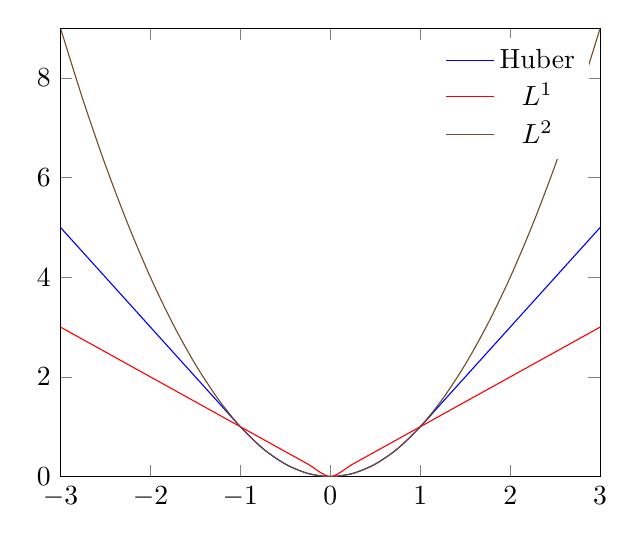
\begin{tikzpicture}
    \begin{axis}[domain=-3:3, enlargelimits = false, legend style={draw=none},cycle list name=color]
        \addplot+[no markers, smooth] { (abs(x)<=1)*x^2 + (abs(x)>1)*(2*abs(x)-1) };
        \addlegendentry{Huber}
        \addplot+[no markers, smooth] { abs(x) };
        \addlegendentry{$L^1$}
        \addplot+[no markers, smooth] { x^2 };
        \addlegendentry{$L^2$}
    \end{axis}
    \end{tikzpicture}
    \caption{Comparaison des pertes Huber, $L^1$ et $L^2$}
\end{figure}

\subsubsection{Gradient Boosting}

Résoudre~\ref{adaboost.eq} est également possible grâce à des méthodes numériques approchées, en effet le programme d'optimisation est
\begin{equation}
    \begin{aligned} \label{gradient.boosting.opt}
        & \text{minimiser}
        & & L(f) = \sum_{i=1}^N  L \left(y_i, f(x_i) \right) \\
        & \text{sous contrainte}
        & & f(x) = \sum_{k=1}^K \beta_k b (x, \gamma_k) \\
    \end{aligned}
\end{equation}

On peut alors appliquer notre procédure de boosting dans le cas plus général d'une perte $L$ différentiable, ainsi la méthode de la descente de gradient est elle-même une procédure gloutonne qui résout~\ref{gradient.boosting.opt} sous la forme:
\begin{gather}
    [g_k]_i = \left[ \frac{\partial L (y_i , f(x_i) ) }{\partial f(x_i)} \right]_{f(x_i) = f_{k-1} (x_i)} \\
    \rho_k = \argmin_{\rho} L ( f_{k-1} - \rho g_k  )
\end{gather}
Et l'approximation courante est mise à jour avec
\begin{equation*}
    f_k = f_{k-1} - \rho_k g_k
\end{equation*}

Cela ne correspond pas exactement à~\ref{gradient.boosting.opt} puisque $f$ doit être contraint, on choisit donc d'entraîner un classifieur sous notre forme contrainte afin d'approcher au plus les valeurs du gradient souhaité. On obtient alors l'algorithme~\ref{gradient.boosting.alg} pour le gradient boosting.

\begin{algorithm}
\caption{Gradient Boosting} \label{gradient.boosting.alg}
\begin{algorithmic}
    \Procedure{Gradient Boosting}{$\mathcal{L}, L$}
    
    \State{$f_0 (x) \gets \argmin_\gamma \sum_{i=1}^N L (y_i , \gamma ) $}
    
    \For{ $k = 1,\dotsc,K$ }
        \State{ $\left[r_m \right]_i \gets - \left[ \frac{\partial L (y_i , f(x_i) ) }{\partial f(x_i)} \right]_{f(x_i) = f_{k-1} (x_i)}$ }
        \State{Entraîne $B_k (x)$ sur les pseudo-résidus $\left\{ (x_i, [r_k]_i \right\}$}
        \State{$\gamma_k \gets \argmin_\gamma \sum_{i=1}^N L ( y_i , f_{k-1} (x_i) + \gamma B_k (x_i) ) $}
        \State{$f_k (x) \gets f_{k-1} + \gamma_k B_k (x)$}
    \EndFor
    \State \Return $f_K (x)$
    \EndProcedure
\end{algorithmic}    
\end{algorithm}

Les arbres de classification présentent d'excellentes performances en tant que classifieur de base pour le boosting, il faut néanmoins porter une attention particulière à leurs tailles afin de pouvoir capturer suffisamment d'interactions entre les variables sans augmenter l'erreur de généralisation.
\todo{Développer sur la taille des arbres en gradient boosting? Sur le Tree boosting en particulier?}

\begin{figure}[htbp]
    \begin{tikzpicture}
    \begin{axis}[domain=0:1, ymin=0, ymax = 1, enlargelimits = false, xlabel = {Taux de faux positifs}, ylabel = {Taux de vrais positifs}, legend style={draw=none,legend pos=south east}]
            \addplot[no markers, const plot, blue] table [x = "fpr", y = "tpr", col sep = comma] {images/roc_boosting.csv};
            \addlegendentry{Boosting}
            \addplot[no markers, const plot] table [x = "fpr", y = "tpr", col sep = comma] {images/roc_arbre.csv};
            \addlegendentry{Arbre seul}
            \addplot[no markers, black, dashed] {x};
    \end{axis}
    \end{tikzpicture}
    \caption{Performances du boosting d'arbres ($\mathrm{AUC} = 0.8103$).}
\end{figure}

\subsection{Stacking}

Nous avons vu plusieurs techniques visant à améliorer les performances d'un classifieur en combinant les résultats de plusieurs classifieurs existants. Néanmoins toutes ces méthodes combinent les résultats de classifieurs issus du même algorithme, une extension naturelle serait alors de créer des classifieurs radicalement différents et combiner leurs résultats pour en obtenir de nouveaux.
Il est alors possible de voir cette seconde étape comme une procédure d'apprentissage machine sur un nouveau \emph{méta} échantillon composé de l'ensemble des prédictions de nos classifieurs. Cette méthode appelée \emph{Stacking} ou \emph{Blending} introduite par \citet{Wolpert1992} a pris de l'importance ces dernières années en présentant d'excellentes performances sur des problèmes industriels réels comme le problème de recommandation de Netflix \citep{Jahrer2009a,Bellkor2008,Bell2007,Jahrer2010}.

Dans \citet{VanderLaan2007a}, les auteurs introduisent un algorithme de \emph{super apprentissage} et montrent que ce nouveau \emph{super classifieur} est asymptotiquement au moins aussi bon que le meilleur des classifieurs le constituant.
Leur algorithme procède en plusieurs étapes:
\begin{enumerate}
    \item L'échantillon d'apprentissage est découpé en $N$ tranches $T_i$ de tailles proches
    \item Pour chaque tranche $T_i$ tous les classifieurs $\varphi_i^j$ sont construits sur l'ensemble $\mathcal{L} \smallsetminus T_i$ et leurs prédictions sur $T_i$ agrégées dans un nouvel échantillon $\mathcal{M}$ avec les vraies étiquettes de chaque individu.
    \item Une fois cette procédure répétée $N$ fois le modèle d'agrégation choisi construit un classifieur $\Psi$ sur $\mathcal{M}$
    \item Chaque classifieur $\varphi^j$ est reconstruit sur $\mathcal{L}$ 
\end{enumerate}
Le super classifieur étant alors $\left\{ (\varphi^1,\dotsc,\varphi^M), \Psi \right\}$

\begin{figure}[htbp]
    \makebox[\textwidth][c]{
        \includegraphics{Superlearner.pdf}
    }
    \caption{Fonctionnement de l'algorithme SuperLearner, adapté de \citet{VanderLaan2007a}}
\end{figure}

Le choix de l'algorithme de meta-apprentissage $\Psi$ influe également grandement sur les performances du super classifieur, il est possible de choisir une fonction aussi simple que le vote majoritaire ou la moyenne non pondérée ou arbitrairement complexe comme un réseau de neurones artificiels profond, le choix étant alors à faire en fonction de jeux de données, de la mesure de performance choisie et le temps de calcul disponible. \citet{Jahrer2010} fournit un aperçu de différentes techniques de mélange et leurs performances.

Ces méthodes de mélange considèrent tous les modèles disponibles quelque soit leur contribution aux performances, pour pallier ce problème et permettre une optimisation de l'ensemble de modèles par rapport à la métrique de son choix. \citet{Caruana2011a} proposent une méthode de construction d'ensemble par étapes où seuls les classifieurs améliorant la qualité de l'ensemble sont rajoutés. En ne prenant comme fonction de mélange que la moyenne, ils permettent des combinaisons très rapides, ce qui autorise l'utilisation de milliers de classifieurs de base. Mais il est tout à fait envisageable d'utiliser un meta classifieur plus performant.

\begin{figure}[htbp]
    \begin{tikzpicture}
    \begin{axis}[domain=0:1, ymin=0, ymax = 1, enlargelimits = false, xlabel = {Taux de faux positifs}, ylabel = {Taux de vrais positifs}, legend style={draw=none,legend pos=south east}]
            \addplot[no markers, const plot, blue] table [x = "fpr", y = "tpr", col sep = comma] {images/roc_stacking.csv};
            \addlegendentry{Stacking NN}
            \addplot[no markers, const plot] table [x = "fpr", y = "tpr", col sep = comma] {images/roc_arbre.csv};
            \addlegendentry{Arbre seul}
            \addplot[no markers, black, dashed] {x};
    \end{axis}
    \end{tikzpicture}
    \caption{Performances du stacking avec réseaux de neurones ($\mathrm{AUC} = 0.7372$).}
\end{figure}

\todo{refaire le diagramme}
\todo{donner exemple, procédure avec Echantillon Train; Echantillon Blend et Echantillon Test}